%!TEX root = ../Thesis.tex
\chapter{Discussion and Future Work}

This chapter further discusses the results from the testing phase, along with plans for future work

\section{Discussion}

The goal of having the thrust vector control restricted to one axis was to allow for the clear understanding of the working principles and process workflow of designing and controlling a rigid body. 
From this understanding, the same principles can be used further, by just extending the rudder to a two-axis control platform instead and adding a decoupled control for the additional axis (yaw). 

The multitude of IMUs tried and tested helped understand the process from the ground up of navigation. From converting the voltage readings into the respective units of each device, to reading and aligning reference frames, to experiencing the limitations of each and relative to each other, such as the errors found in the cheaper versions (crosstalk) were significantly reduced in the higher end ones (BNO055). It was not the initial plan to test multiple IMUs, however as more sensors became available, it warranted comparison for finding the better fit for the project. 
The initial recommendation from the organisation was to limit the scope of this project by simulating a perfect IMU sensor.
This was to avoid dealing with the significant challenges of real-world hardware. However, the navigation has proven to be a highly rewarding phase in terms of understanding the process, real life challenges in inertial sensors and the interaction with hardware.  
 
Before finding the Mahony/Madgwick filters, there were other filters tried, which were finally deemed insufficient on their own compared to these filters - since both Mahony and Madgwick handle vibration well. There is however a noise component to the navigation output of these filters, which is detrimental to the Derivative of the PID controller. 
Multiple methods for removing noise were tried, such as Moving Average with different weight for older versus newer data, Weighted average, Median filter, Savitzky-Golay Filter, out of which Moving Average filters showed the most promising results, as they have an effect of smoothing the errors, whereas Savitzky-Golay proved to follow outliers more closely as opposed to removing them. 
Moving average is a Finite Impulse Response (FIR) filter, taking N data samples and averaging them over a given window of time. 
Exponential moving average filter is an Infinite Impulse Response (IIR) filter. It has a parameter (weight) ranging from 0 to 1, a higher value giving more weight to older data. In figure  \ref{movingaverage}, this parameter was set to 0.9. 

\begin{figure}[H]
  \centering
  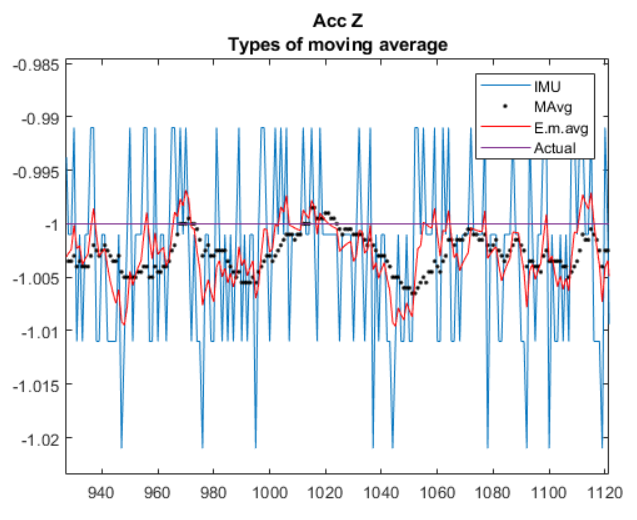
\includegraphics[scale=0.7]{graphics/accZ.png}
  \caption{Comparison of moving average filters}
  \label{movingaverage}
\end{figure}

Figure \ref{movingaverage} shows the noise of an accelerometer in one axis (z), measured in units of g (9.8 m/$s^2$). This graph plots the acceleration (y axis) measured while the sensor is maintained static, over a subset of samples taken (x axis).
The red line ("Actual"), represents the true value of the gravitational acceleration, 1 g, used as reference. The blue "IMU" signal represents the noisy IMU measurement of the gravitational acceleration. The signals plotted in red and black show the two types of moving average filters, sliding window and exponential weighting.

While the exponential method follows the changes in signal more precisely, sliding window moving mean provides a smoother signal, that is more suitable for passing the data to a controller, as is the case in this project. Therefore, the sliding window method would be preferred. 
It can be noticed that the moving average introduces a delay, significant compared to the exponential moving average. The moving mean filter of length N has a sample delay of:

\begin{equation}\label{delay}
	(N-1)/2
\end{equation}

An attempt was made to compare simple moving average and exponential weighted moving average filters from figure \ref{movingaverage} between themselves, with delay removed from the simple moving average. In that effect, it can be seen in figure \ref{movingaveragenodelay} that the smoothing effect is slightly improved over the exponential moving filter, achieving lower peaks and more cohesive data. The moving average filter can be a useful alternative to the complementary filter-based solutions presented in the fusion chapter, if the delay is taken into consideration. Measurement data was found to be normally distributed, therefore the IMU could also benefit from a probabilistic filter such as Kalman filter, given sufficient processing power. 

\begin{figure}[H]
  \centering
  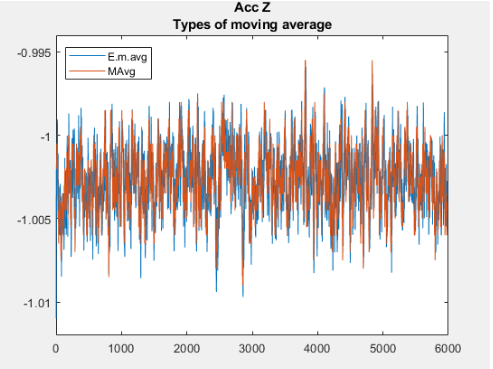
\includegraphics[scale=0.9]{graphics/accznodelay.png}
  \caption{Comparison of moving average filters with removed delay}
  \label{movingaveragenodelay}
\end{figure}

The complementary filter was found to be an insufficient solution for the purpose of rocket flight due to its estimation capabilities - however, even if it were to have had better performance, it remains unsuitable due to singularities occurring in its Euler angles calculations. Mahony and Madgwick filters are expected to have improved performance with more stable calibration of the sensor. Madgwick filter could be tuned to give higher weight to the accelerometer and magnetometer data in order to be more stable, however, that also introduces slower convergence time. 
On top of that, however, there is further need of smoothing the signal and applying a filter like the Moving Average, with delay compensated for, in order to not impact the controller - for example, in the PID's Derivative gain. 

Due to software errors, it was not possible to test the controller with the navigation filters found in this project, instead having tested with the stock in-built navigation solution of the IMU. Future work will include tests with Mahony and Madgwick filters.   
Calibration of the errors was important because the derivative component of the PID amplifies high-frequency signals (noise) in the sensor measurements.
This was evident during the tests performed on IMU without the filters discussed in this section, but with its stock calibration instead. The Derivative term was nearly unusable. 
In case of using the Integral part of PID, anti-windup measures are also necessary, however, due to its possible complications, the intention was to not implement this component. 
There was a clear difference, even for model-based control, between simulations and real-life hardware response. The difference could be attributed to many factors - imprecision of parameters fed into the model (such as calculated moments of inertia), not having accounted for delays in actuator response and battery consumption, significantly noisier data than the simulated signal. This could potentially be improved by designing a controller and testing it with simulated noisy data and also with input of the IMU sensor noisy data. 

Working with hardware as opposed to simulated data has been particularly rewarding, especially due to the challenges it brings. Familiarizing with IMU sensor data has been particularly difficult, but a very important learning component regarding measurements and their true output requirements. Testing on real-life devices has helped visualise the true response of systems under different inputs, as well as the difference from the expected outcome.



\section{Future work}

This chapter rounded up the remaining discussion of the project.
Subsequent iterations of the hardware prototype would expand its capabilities to two axis control surface, which would require designing and building another deflection mechanism.

Future tests will include the navigation methods found in this project along with the controller.  
The navigation will be tested on a small scale rocket built by former DanSTAR students of DTU, in collaboration with Copenhagen Suborbitals, planned to be launched in Portugal in the fall of 2021. Prior to this, there will be conducted additional vibration tests of the filters, along with performance under acceleration, jerky movements and heavy vibration. 
The controller will have added features with focus on robustness and adding variable mass and moment of inertia as opposed to the fixed bodies moment of inertia in the current iteration. Tests should be done on variable mass drone to closer simulate the rocket. Since the system is fully controllable, tests could be performed with a placed set of stabilizing eigenvalues and compare performance against the PID.  
Another possibility for control architecture is gain scheduling or cascaded control, an industry-proven solution for rocket control. 
An LQR controller was also designed and simulated, however, its output was maintaining the system marginally stable and oscillating, as opposed to dampening its oscillations. Further inquiring into its behavior will be made before it will be applied on the UAV and tested against the PID.
